\section{Nytorv før 00'erne}
\label{sec:nytorv_foer_null}
Nytorv er et af samlingspunkterne i Aalborg , og der færdes mange mennesker og køretøjer dernede. Bevirker det, at cyklister og fodgængere føler sig utrygge dernede? Og hvordan kan man i det hele taget modvirke, at der sker konflikter mellem dem på Nytorv. Det er spørgsmål, som bliver undersøgt i denne rapport.
<<<<<<< HEAD
Tilbage i 1980 vedtog det i Aalborg kommune en arealanvendelsesplan for Aalborg Nytorv. \autocite{Madsen2010}
=======
Tilbage i 1980 vedtog man i Aalborg kommune en arealanvendelsesplan for Aalborg Nytorv. \autocite{arealplan}
>>>>>>> 5c1ac62b1c9e7598022477d33235f6cb2de4ee8e
%(http://apps.aalborgkommune.dk/images/teknisk/PLANBYG/lokplan/01/10-010.pdf (s. 2))
Formålet med denne plan, var at gøre Nytorv til et såkaldt ”bybånd”, altså en bykerne med et godt trafik flow, med særlig hensigt på en kollektive trafik. I trafikplanen var en af tingene at etablere et buscenter, som skulle strække sig fra omkring det nuværende Algade ned til Nytorv og op til Slotsgade, hvor der så kun måtte køre busser. Strækningen er illustreret som den gule rute på figur \cref{fig:midtby} side \pageref{fig:midtby}.
\begin{figure}[htbp]
   \centering
   \begin{adjustbox}{max width=\textwidth}
     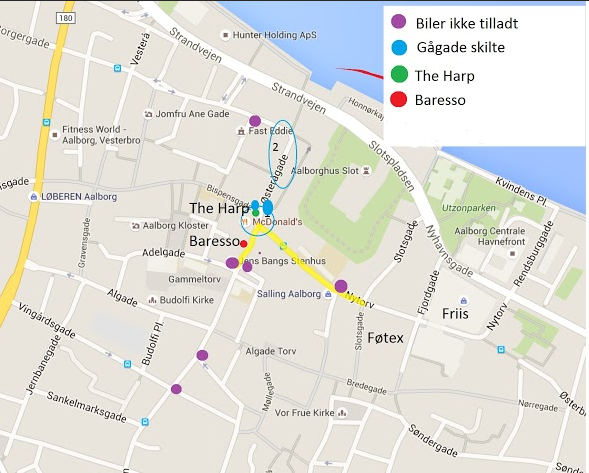
\includegraphics[scale=0.3]{figures/Billederogfigur/midtby.jpg}
  \end{adjustbox}
   \caption{Kort over Aalborg midtby \autocite{gm2015}}
   \label{fig:midtby}
 \end{figure}
Det skulle gøre det nemmere for busserne, at komme hurtigere frem i trafikken\autocite{arealplan}. Det  væsentlige hovedformål, taget ud fra en redegørelse af den daværende trafikplan, var :
”at der skabes bedre omstigningsmuligheder, dels mellem bybusserne     indbyrdes, dels mellem bybusser og rutebiler.”
%(http://apps.aalborgkommune.dk/images/teknisk/PLANBYG/lokplan/01/10-010.pdf (s. 3))
Det var altså en plan for at gøre det lette tilgængeligt for bybusserne at transportere sig rundt i bymidten, uden at skulle konflikteres med den individuelle trafik. Dermed også gøre det hurtigere som borger, at transportere sig rundt i Aalborg.
I 1998 sker der så en omlægning af Østerågade/Nytorv \autocite{omlaegning}.
%http://www.trafikdage.dk/td/papers/papers00/Dag1/paper/1203.pdf (s. 85))
Nytorv blev omlagt således, at granitbelægningen blev ens både på fortov og vej. Vejbredden blev gjort mindre, og det lyskryds der var på Nytorv, blev til og med fjernet. Nytorvs struktur gik altså fra et mere opdelt fortov/trafikvej, hen mod et såkaldt ”Shared space”. Begrebet Sharedspace vil blive beskrevet mere detaljeret senere i rapporten. En af ændringerne fra trafikplanen i 1980 var, at nu måtte kun biler med ærinder, busser og erhvervsbiler køre ind på området omkring Nytorv. Adgang for biler på Nytorv var altså nu forbudt. Udfaldet af dette var et fald af den private bilkørsel på Nytorv med ca. 60 procent \autocite{omlaegning}.
%(Der er en tabel i et link Bjørn har, som viser det)
Meningen med at forhindre den private bilkørsel, var at gøre Aalborg bymidte til et sted, hvor der var gode vilkår for cyklister, fodgængere og den kollektive trafik. Det skulle være lettere at transportere sig rundt på cykel og gåben, da Nytorv nu var et fællesareal, hvor det udelukkende var cykler, fodgængere og busser der færdes.
